\documentclass[sii]{ipart}

\RequirePackage[OT1]{fontenc}
\RequirePackage{amsthm,amsmath}
\RequirePackage[numbers,square]{natbib}
\RequirePackage[colorlinks]{hyperref}
\usepackage{caption}
\usepackage{booktabs}%table
\usepackage{multirow}%table
\usepackage{graphicx}%figure
\usepackage{amssymb} %hollow character 



% settings
\pubyear{0000}
\volume{0}
\issue{0}
\firstpage{1}
\lastpage{8}

\startlocaldefs
%\numberwithin{equation}{section}
\theoremstyle{plain}
\newtheorem{thm}{Theorem}[section]
\endlocaldefs

% will be filled by editor:
\pubyear{0000}
\volume{0}
\issue{0}
\firstpage{1}
\lastpage{1}
%\arxiv{}

%set work directory
\graphicspath{{/Users/daniel/Documents/-Work/20181122/20181122UBI/deliver/}}

%\graphicspath{{/users/zhangyuxuan9511/Documents/essay/UBI/deliver/}}
%\graphicspath{{/users/yuxuan/Documents/essay/UBI/20181120UBI/deliver/}}

\begin{document}
	
	\begin{frontmatter}
		
		% "Title of the Paper"
		\title{Usage Based Insurance Model with Point of Interest Data}
		%\title{UBI\thanksref{t1}}
		\thankstext{t1}{Yuxuan Zhang, Jinchang Fan and Rui Pan are from School of Statistics and Mathematics, Central University of Finance and Economics, Beijing, 100081, P. R. China. Liang Huang is from CIHON (Beijing) New Technology Co., Ltd., Beijing, 110000, P. R. China. The research is supported in part by National Natural Science Foundation of China (NSFC, 11601539, 11631003).}
%		\runtitle{???}
		
		% indicate corresponding author with \corref{}
		 %\author{\fnms{John} \snm{Smith}\thanksref{t2}\corref{}\ead[label=e1]{smith@foo.com}\ead[label=e2,url]{www.foo.com}}
		% \thankstext{t2}{Thanks to somebody}
		% \address{line 1\\ line 2\\ \printead{e1}\\ \printead{e2}}
		
		\author{\fnms{Yuxuan} \snm{Zhang}},
%		\address{\printead{e1}},
		\author{\fnms{Jinchang} \snm{Fan}\thanksref{t2}\corref{}},
		\author{\fnms{Rui} \snm{Pan}}
		\and
		\author{\fnms{Liang} \snm{Huang}}
		\thankstext{t2}{Corresponding author.}
		%\address{???\printead{e2}}
		
		\runauthor{}
		
\begin{abstract}
With the rapid advance of the Internet of Vehicles (IOV), IOV data are becoming 
increasingly available. This kind of data includes plentiful information, which can reflect driving behavior and driving environment. In this work, we try to utilize IOV data for accident prediction. Specifically, we propose a Usage Based Insurance (UBI) model where the response is whether the vehicle is involved in an accident.
Mileage, driving behavior as well as Point of Interest (POI) information are incorporated as predictive variables. The estimated model can be further used for driver segmentation.
\end{abstract}
		
		%\begin{keyword}[class=AMS]
		%\kwd[Primary ]{}
		%\kwd{}
		%\kwd[; secondary ]{}
		%\end{keyword}
		
		\begin{keyword}
		\kwd{Internet of Vehicles}
		\kwd{Point of Interest}
		\kwd{Usage Based Insurance}
		\end{keyword}
		
		% history:
		% \received{\smonth{1} \syear{0000}}
		
		%\tableofcontents
		
	\end{frontmatter}
\section{INTRODUCTION}

In the past decade, the whole world witnessed the tremendous development of vehicle industry. According to the statistics published by the International Organization of Motor Vehicle Manufacturers ({\it www.oica.net}), 97,303 thousands of motor vehicles are produced in 2017 all over the world. In addition, it is projected that there will be around 1.1 billion passenger vehicles by 2030 \cite{lee2011will}. The flourish of vehicle industry brings a brand new field, the Internet of Vehicles (IOV). Vehicles equipped with specific communication instruments are incorporated in the IOV. As a result, IOV gathers data from vehicles and makes sure the fulfillment of information communication, environmental protection, energy conservation and safety \cite{liu2011internet}.


In-vehicle data recorders (IVDR) are one of the general resources for IOV data. Thanks to IVDR and various sensors, ample data could be collected from vehicles. These data include but are not limited to, vehicle location, velocity, acceleration, mileage, and engine parameters such as fuel consumption, engine rotation speed, and many others. In the rest of this article, we refer to the data collected by IVDR as IOV data. It is noteworthy that IOV data are typically recorded every second and contain plentiful information in great detail. This leads to large scale of the data, which might be thorny for analysis. For example, the data adopted in this work contain multifarious information of 1,453 cars, accumulating records approximate 14 million kilometers.

Statistical analysis of IOV data could be widely used in different fields, contributing to transportation department, drivers, and insurance business. For instance, collision avoidance technologies could serve to reduce the chance of accident by collision warning system and driver assistant system \cite{fangchun2014overview, mclaughlin2008method}. In addition, drivers could attain better driving experience by finding local services more conveniently \cite{fangchun2014overview, karagiannis2011vehicular}. Another important application of IOV data lies in actuarial decision-making. Insurance companies could profit by offering more reasonable insurance products for policyholders. One of the most prevalent insurance products is Usage Based Insurance (UBI).


UBI is an innovative insurance product, where the premiums are based directly on how much the vehicle is driven during the policy term \cite{litman2011distance}. This kind of insurance is economical, because drivers are encouraged to mind their behavior in order to save money. In addition, UBI attracts growing interest, since it achieves additional social benefits including traffic safety and environmental objectives \cite{bolderdijk2011effects, parry2005pay}. Some insurance companies now offer UBI options, e.g., Progressive ({\it https://www.progressive.com}),  Insure The Box ({\it https://www.insurethebox.com}), and many others. Nevertheless, UBI could not be implemented without IOV data. IOV data provide information on usage and driving behavior, which are the basis of UBI pricing. By analyzing IOV data, the accident prediction model is established and the probability of accident could be calculated \cite{paefgen2014multivariate, wu2012crashes, ayusoanalyzing}.



Generally, there are two types of work on UBI study. The first type only considers mileage as the explanatory variable. Literature includes analyzing the relationship between mileage and accident occurrence \cite{lourens1999annual}, mileage and crash fatalities \cite{litman2011distance} as well as mileage and insurance claims \cite{bordoff2008pay, ferreira2010pay}. Later, nonlinear relationship particularly for low-mileage drivers is further studied \cite{staplin2008low, langford2008defence}. Recently, mileage is proved to be a significant predictor of accident cost \cite{ferreira2012measuring}. Mileage and other classic rating factors together will improve explanatory power significantly. The second type of research takes vehicle velocity into consideration \cite{kloeden2002reanalysis, jun2007relationships, brijs2006impact}. It is demonstrated that driving performances concerning braking and acceleration are significant in distinguishing drivers involved in crashes \cite{jun2007relationships}. Various statistical models are adopted in these studies, including Poisson log-linear model \cite{gordon2011analysis}, exponential-type model \cite{ayusoanalyzing}, and many others  \cite{paefgen2014multivariate, paefgen2013evaluation}.


Although plentiful works concerning UBI have been conducted, several shortcomings still exist. First of all, the sources of data are limited. Two main sources are Virginia Tech Transportation Institute and US Strategic Highway Research Program. As for dataset provided by Virginia Tech Transportation Institute, it merely contains records of 100 vehicles \cite{dingus2006100}. Second, only GPS observations are available in most of these data, which may cause inaccuracy in calculating velocity and acceleration. On contrary, data recorded by sensors from IVDR are relatively accurate and reliable. Third, predictors used in those works are lack of diversity. Only vehicle information (e.g., mileage and velocity) and driving behavior (e.g., the proportion of drowsy driving) are taken into consideration. Nonetheless, important information derived from location data and trajectory data is neglected.

In our work, improvements are achieved in all the three aspects. Dataset used in this work are offered by a famous vehicle manufacturing group. Detailed and diverse information regarding vehicles is included, providing much evidence of driving behavior. In addition, IVDR records vehicle velocity and acceleration through specific sensors so that the accuracy of data is warranted. At last, Point of Interest (POI) data are considered in this work. It will be discussed below that POI data contain plentiful information concerning driving behavior and environment.


POI is a specific point location which might be useful or interesting to someone. It includes spots such as sightseeing sites, gas stations, restaurants and many others. POI data could be uploaded by users of social networking and online advertising applications like Facebook, Weibo, and Yelp. A piece of POI data normally consists of name, latitude, and longitude of a location. Tags, categories, and other information are also frequently attached to POI data \cite{chenyu2017poi}. Furthermore, POI data have a wide range of applications. For example, POI recommendation could be utilized to suggest living facilities, bus stations, restaurants, etc. \cite{yuan2013time, liu2013learning}. Another application of POI data is pattern identification of population flow \cite{veloso2011urban, noulas2011empirical}. Human daily patterns could be analyzed and discovered through POI data. As for UBI, POI data provide us with a new perspective on predicting accidents since they could reflect driving environment. In fact, several existing pricing strategies including GPS-based pricing have already taken environment into consideration \cite{litman2007distance}. For instance, it is conceivable that accident is less likely to happen during a trip to a national park, since roads toward national parks are typically uncrowded.

The rest of this article is organized as follows. In Section 2, we introduce our IOV and POI data, together with brief descriptive analysis. In Section 3, logistic regression is applied to build the UBI model. Estimation and prediction results are explained in detail. Some business applications are further discussed in Section 4. Some concluding remarks are given in Section 5.


\section{DATA DESCRIPTION}
\subsection{The IOV Data} 
In this paper, data are provided by a major Chinese automobile manufacturer, recorded by IVDR. Data are collected from 1,453 vehicles, ranging from September 2014 to September 2015. The data cover more than 14 million kilometers in total. Insurance records are also included in the dataset. It is a binary variable indicating whether the vehicle has reported accident (for 1) or not (for 0). There are 49.6\% drivers reported accident in our data.  Vehicles are identified by Vehicle Identification Number (VIN) and all private information is protected. 

IVDR collects and updates records every second and consists of the following information:
\begin{itemize}
	\item VIN: unique identification number for each vehicle. It is the only identification of a vehicle, which includes no private information, e.g., LLNC1AAA2EA00****.
	\item  Time of record: time stamp of data recorded by IVDR, e.g.,  2015-02-12 16:32:48. The interval between adjacent record is one second.
	\item Latitude \& Longitude: instantaneous position of a vehicle. The accuracy of position is around ten meters. The latitude and longitude provide us with the position of a vehicle and POIs near it could be scanned.
	\item Mileage: accumulated mileage of vehicle till the time point we observe, ranging from 629 to 26,690 kilometers. The mileage is generally adopted as a crucial predictor in UBI. The larger the mileage, the more likely a vehicle is involved in an accident.
	\item Fuel consumption: instantaneous fuel consumption, measured by liters per 100 kilometers ($L/100 \, km$). Higher instantaneous fuel consumption might be related to acceleration or other behavior, thus reflecting driving behavior.
	\item Velocity: instantaneous velocity of a vehicle, ranging from 0 to 220 kilometers per hour ($kph$). It is automatically calculated from detected revolution (rev) of wheels.
	\item Acceleration: longitudinal acceleration, detected by gyroscope that could diminish the influence of tilt when vehicle is on slope. A positive record indicates the vehicle is accelerating and a negative record indicates the vehicle is decelerating. The unit of record is meter per second squared ($m / s^{2}$). 
	\item  Engine rev: instantaneous engine rotational speed, ranging from 0 to 4,000 revolutions per minute ($rpm$). It indicates the instantaneous power of engine. The engine rev is related to vehicle velocity. However,  considering that it takes the size of gear as a multiplier, the relationship is more complicated than linear relationship. 
	
	
	
	
\end{itemize}
\begin{figure*}[t!]
	\centering

	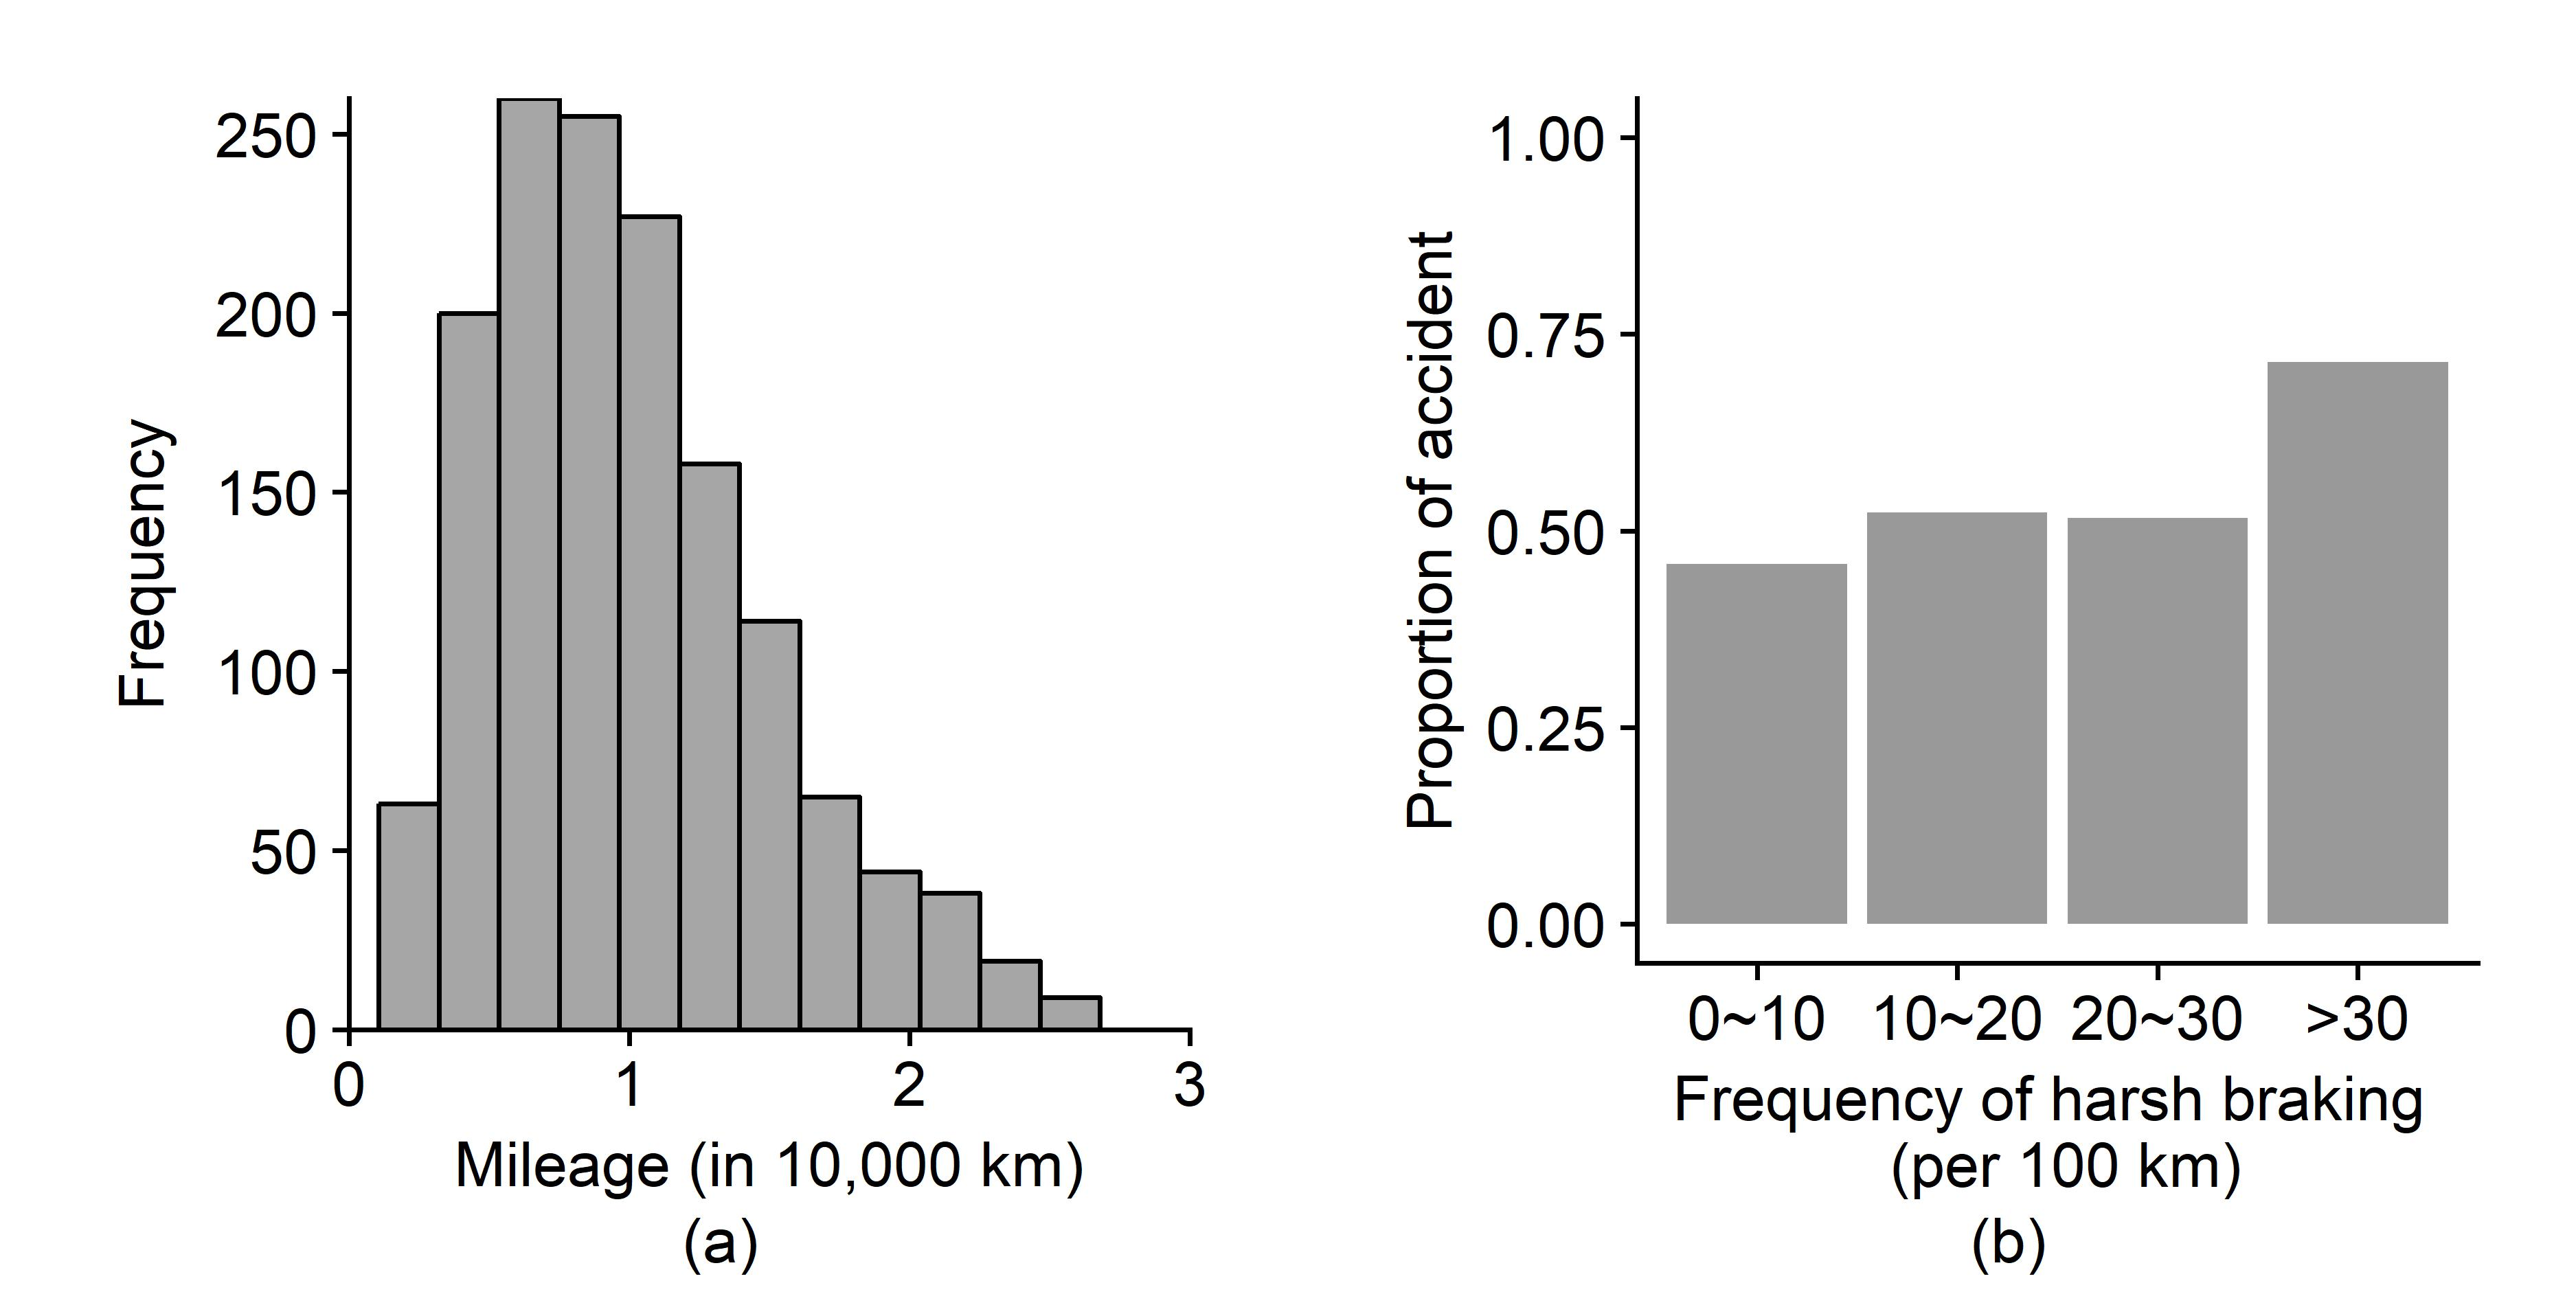
\includegraphics[width=0.7\linewidth]{hist_mileage&y_brake}
	\small\caption{Figure (a): histogram of mileage. A right skewed shape can be detected, indicating the existence of extreme large values in mileage. Figure (b): proportion of accident in different groups of harsh braking frequency. Accidents happen more for those who make harsh breaking more than 30 times per one hundred kilometers.}
	\label{fig:histmileage}
\end{figure*}

\subsection{Descriptive Analysis} 
We next conduct descriptive analysis on the IOV data. Figure \ref{fig:histmileage} (a) shows the histogram of mileage of all vehicles. The mileage ranges from 629 to 26,690 kilometers, with an average of 9,978 kilometers. It is obvious that mileage is right skewed, which indicates that a few vehicles run extremely long distance. Figure \ref{fig:histmileage} (b) divides drivers into four groups according to their harsh braking habits. The height of the bar indicates the proportion of accidents within each group. As it is shown, frequency of harsh braking could serve as a predictor for accident prediction.





In the rest of this work, we define a trip as a consecutive driving behavior from a start to a destination. Figure \ref{fig:path} (a) represents the path of a trip, according to latitude and longitude recorded by IVDR. Note that the exact records of position are much denser than points shown in the figure, but simplified for clearer distinguish. Accumulative mileage, velocity, and acceleration are also presented in Figure \ref{fig:path}. Data recorded every second could bring more insight for us. For example, abnormal driving behavior like harsh braking and rapid acceleration can be accurately detected.

\begin{figure*}[h!]
	\centering
	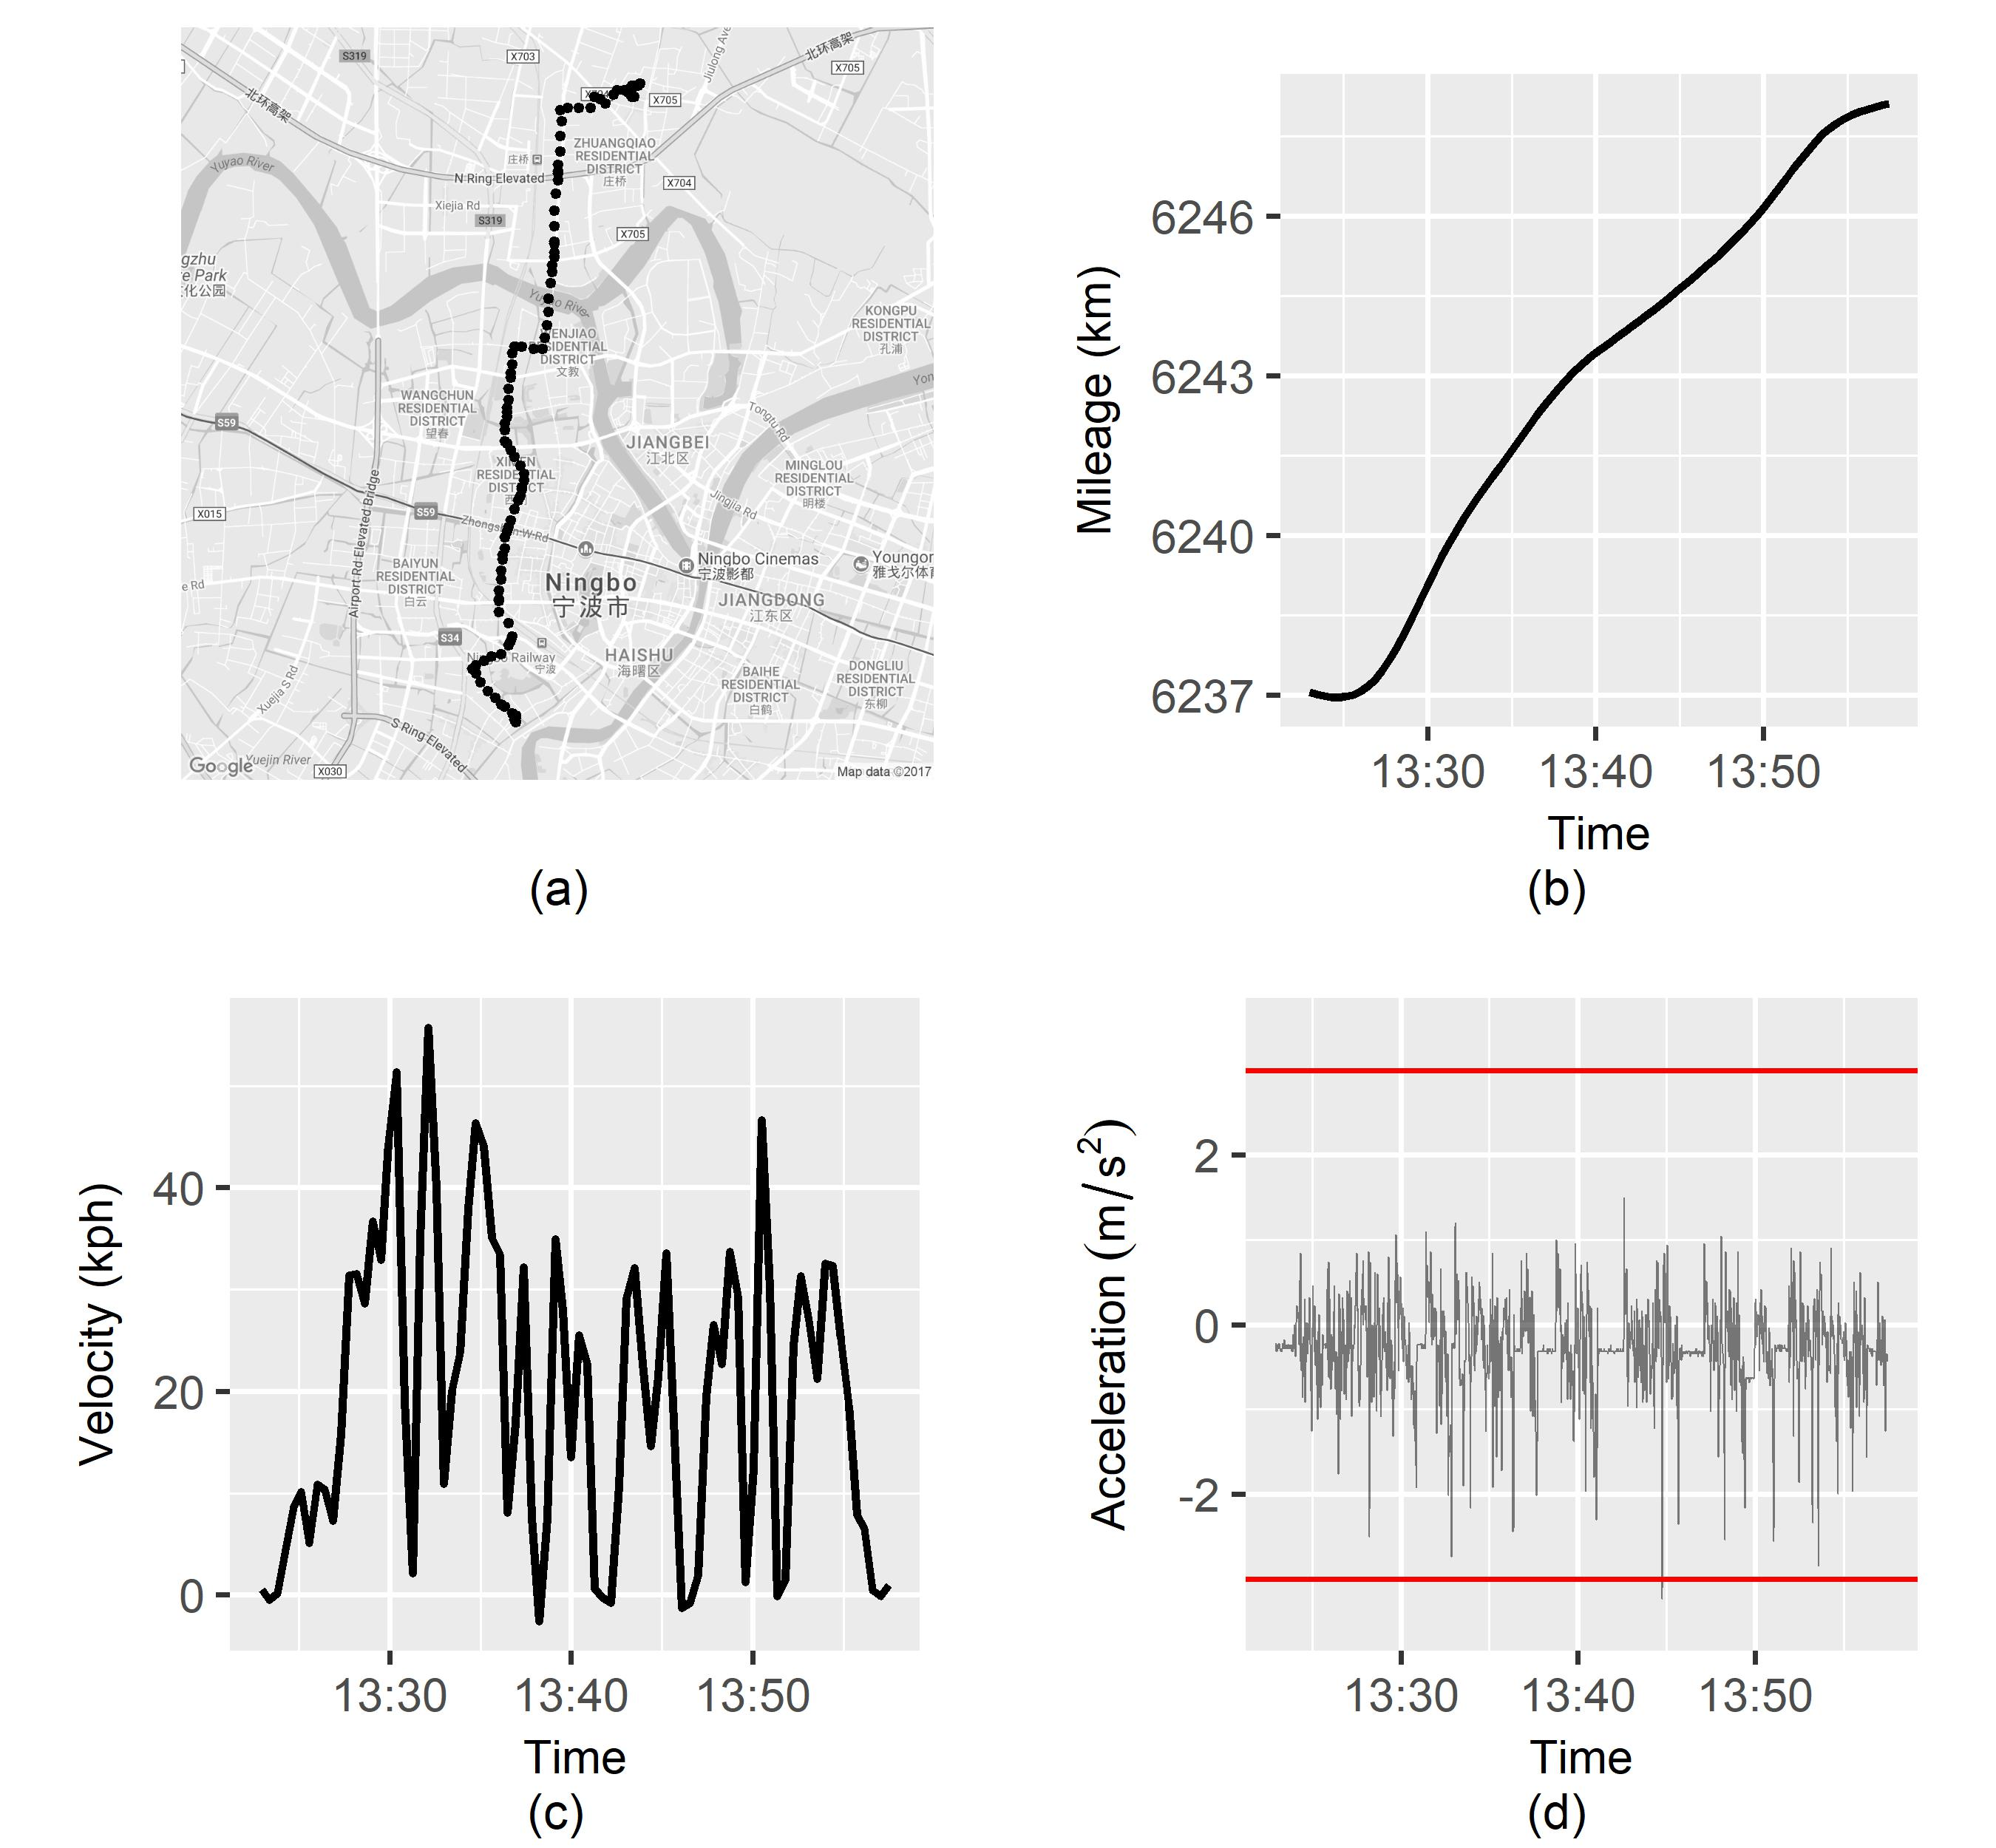
\includegraphics[width=0.7\linewidth]{trace}
	\caption[]{A sample trip. Figure (a) shows the path of the trip. It started from Jiangbei District and went south to Haishu District, experiencing 11 kilometers and around 35 minutes. Figure (b) and (c) show the time series of mileage and velocity of the vehicle during this trip. Low points in (c) indicate several periods of waiting at intersections. Figure (d) shows the time series of acceleration, and two red horizontal lines indicate $3$ and $-3 \, m/s^2$, which are considered as benchmarks of rapid acceleration and harsh braking. }
	\label{fig:path}
\end{figure*}

\subsection{The POI Data}

POI data adopted in this work are from Sina Weibo's open API ({\it http://open.weibo.com}), where Sina Weibo is one of the largest social media platforms in Chinese. The POI data contain POI information uploaded by users of Sina Weibo, including positions, names, categories, etc. Since a POI always contains latitude and longitude, it indicates a point on the map, which is illustrated in Figure \ref{fig:poimap}.
For simplification, we classify POIs into 117 different categories based on the criterion provided by Sina Weibo's open API. 

%In order to derive POI predictors, we first get check-in matrix
% $$C_i=(c_{k,l}) \in \mathbb{N}^{trip_i \times 117}$$
% for each vehicle $i$, where $c_{k,l}$ is the number of POIs in category $l$ are detected around the destination of trip $k$, with  500 meters radius of scanning POIs, and $trip_i$ is the total number of trips of vehicle $i$.
%Then, POI design matrix $X^{POI}=(X_1^{POI}, \dots ,X_n^{POI})^\top$ that represents frequencies of each POI categories for each vehicles is acquired, where
%\begin{equation} 
%X_i^{POI}=(\frac{1^\top C_i}{trip_i})^\top.\label{eq:XPOI}
%\end{equation} 
For each trip of a vehicle, the position of the destination is derived. Next, all POIs within 500 meters of the destination are scanned and the number of POIs is counted within each POI category. For instance, there are three restaurants, one residential area and one school within 500 meters of the center of Figure \ref{fig:poimap}.
%Results for all trips of one particular vehicle are averaged to attain POI data of this vehicle. Thus, the frequencies of each POIs for each vehicle are derived.
We will introduce rigorous mathematical formulas and discuss how POI information is further made use of in the next section.

%It is shown in the data that mean frequency of all POI categories in all vehicles is 0.320, which indicates that each POI category appears 0.320 time on average in each trip. The most welcomed POI category is Residential area.Restaurant with mean frequency of 3.422. On the contrary, the least welcomed one is Pet supply store.Building gate with mean frequency of 0.001. 
%According to the POI data, the mean frequency of all POIs in all vehicles is 0.320, which indicates that each POI appears 0.320 time on average in each trip. The most welcomed POI is Residential area.Restaurant with mean frequency of 3.422. On the contrary, the least welcomed POI is Pet supply store.Building gate with mean frequency of 0.001. We will discuss how POI information is further made use of in the next section.



\begin{figure}[h!]
	\centering
	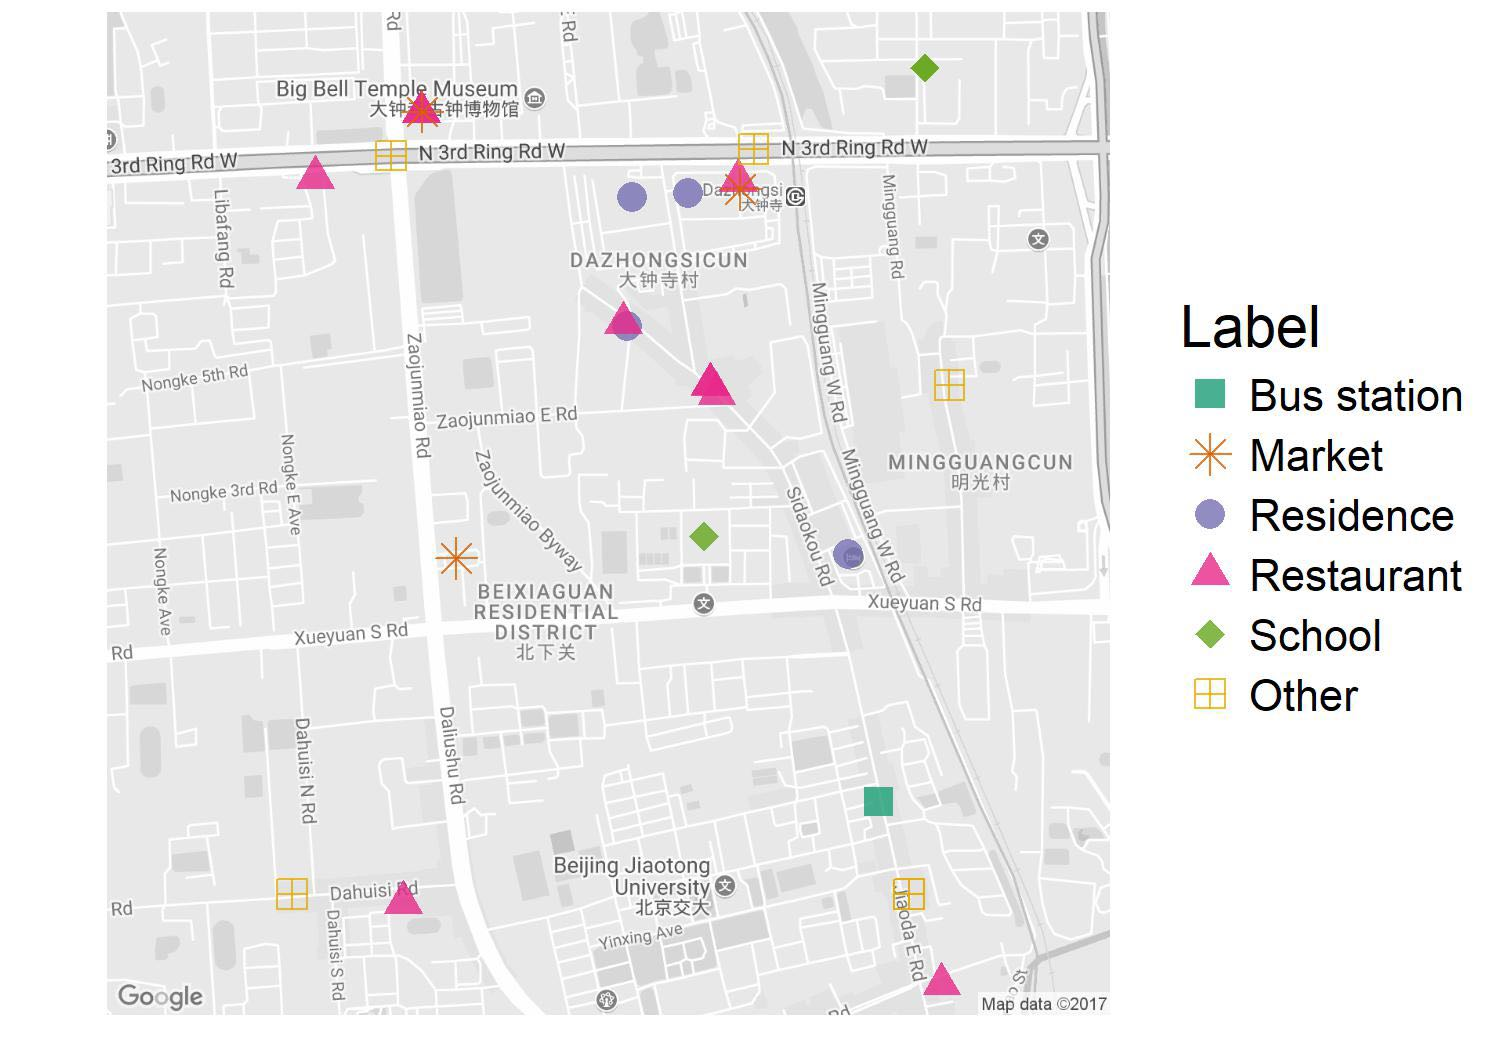
\includegraphics[width=1.\linewidth]{poimap}
	\small\caption[]{An instance of map with POI. Different shapes and colors indicate different categories of POI, including bus station, restaurant, school, etc.}
	\label{fig:poimap}
\end{figure}





\section{Usage Based Insurance Model}

The major concern of this work is to discern drivers with different probability of accident involvement. Logistic regression model is adopted to score each driver based on their driving behavior and POI data. Let $Y_i \in \{0,1\}$ represents the response, where $1 \leq i \leq n$, and $n$ is the total sample size. If $Y_i = 0$, the $i$th vehicle did not report any accident or insurance claim during the observed period, otherwise $Y_i = 1$. Let $X_i = (x_{i1}, \dots ,x_{ip})^\top \in \mathbb{R}^p$ be the covariate vector. The probability of binary response variable $Y_i$ to be one is modeled as
\begin{equation} 
Y_i \sim Bernoulli(p(X^\top_i\beta)),\label{eq:model}
\end{equation} 
where $\beta=(\beta_1,\cdots,\beta_p)^\top\in \mathbb{R}^p$ is the $p$-dimensional regression coefficient, and $p(t)=e^t/(1+e^t)$ is logistic link function, which keeps the probability lying between 0 to 1. In addition, maximum likelihood estimation is conducted, which is denoted as $\hat{\beta} \in \mathbb{R}^p$


In most existing literature, only IOV data are incorporated in the model. Our model incorporates both IOV data and POI data in order to heighten the prediction accuracy. To obtain a more comprehensive understanding, stepwise approach and Akaike information criterion (AIC) \cite{akaike1987factor} are adopted, since not all predictors are significant.



\subsection{The Construction of Predictors} 
Based on the raw data, 10 IOV predictors are derived, as well as 117 POI predictors. Those predictors could be divided into four categories: usage, stability, driving period and POI (Table \ref{tab:Predictors}). 

\subsubsection{The IOV predictors}
IOV predictors including variables in usage, stability and driving period categories. In usage category, accumulative mileage $x_{i1}$ measures the exposure feature of the vehicle $i$ \cite{wolfe1982concept}, and other predictors ($x_{i2},x_{i3},x_{i4}$) are calculated as the arithmetic mean of observed data. In stability category, steer position $x_{i5}$ is calculated as standard deviation. That is, for $i=1, \dots ,n$, $2 \leq j \leq 5$,
$$x_{ij}=\frac{\sum_{k=1}^{t_i} s_{ij}^k}{t_i},$$
where $s_{ij}^k$ is the mean or standard deviation of $j$-th variable in trip $k$ for vehicle $i$, and $t_i$ is the total number of trips for vehicle $i$. 
Frequency of rapid acceleration $x_{i6}$ and harsh braking $x_{i7}$ are the number of instant longitudinal accelerations over $3 \, m/s^2$ or less than $-3 \,  m/s^2$ respectively. Predictors in driving period category is the number of trips occurred during certain time periods. IOV predictors are standardized in model estimation. The original data are shown in Table \ref{tab:Predictors}.		

\newcommand{\tabincell}[2]{\begin{tabular}{@{}#1@{}}#2\end{tabular}}
\begin{table*}[h]
	\caption{Predictors involved in different categories (i.e., usage, stability, driving period and POI)}\label{tab:Predictors} 
	\vspace{0.5ex}
	\begin{tabular}{cllll} 
		\toprule[1pt]
		\toprule[1pt]
		Category & Variable Name & Unit & Range & Detail\\
		\midrule[1pt]
		\multirow{4}*{Usage}&$x_{i1}$ (Accumulative mileage) &km &629-26690 &\\
		&$x_{i2}$ (Average velocity)& kph & 13.30-40.57 & \\
		&$x_{i3}$ (Average fuel consumption) &L/100 km&4.67-8.08 &\\
		&$x_{i4}$ (Average engine rev)& rpm &1019.00-1459.91 &\\
		\cline{2-5}
		\multirow{3}*{Stability}&$x_{i5}$ (S.D. of steer position)& &52.49-123.37 &\\
		&$x_{i6}$ (Frequency of rapid acceleration)  & &0-2.65 &Times per 100 kilometers\\
		&$x_{i7}$ (Frequency of harsh braking)  &  &  1.45-35.90 &Times per 100 kilometers\\
		\cline{2-5}
		\multirow{3}*{Driving Period}&$x_{i8}$ (Count of trips in morning)& &7-294 &From 7:00 to 10:00\\
		&$x_{i9}$ (Count of trips in evening)&&2-329 &From 17:00 to 19:00\\
		&$x_{i10}$ (Count of trips at night)&  & 0-53 &From 0:00 to 4:00\\
		\cline{2-5}
		POI &\tabincell{l}{$x_{ij}$ (Residential area, Bus station, \\  Entertainment, Hospital, etc.)} && &$11 \leq j \leq 127$\\
		\bottomrule[1pt]  
	\end{tabular}
\end{table*}  

\begin{figure}[h!]
	\centering
	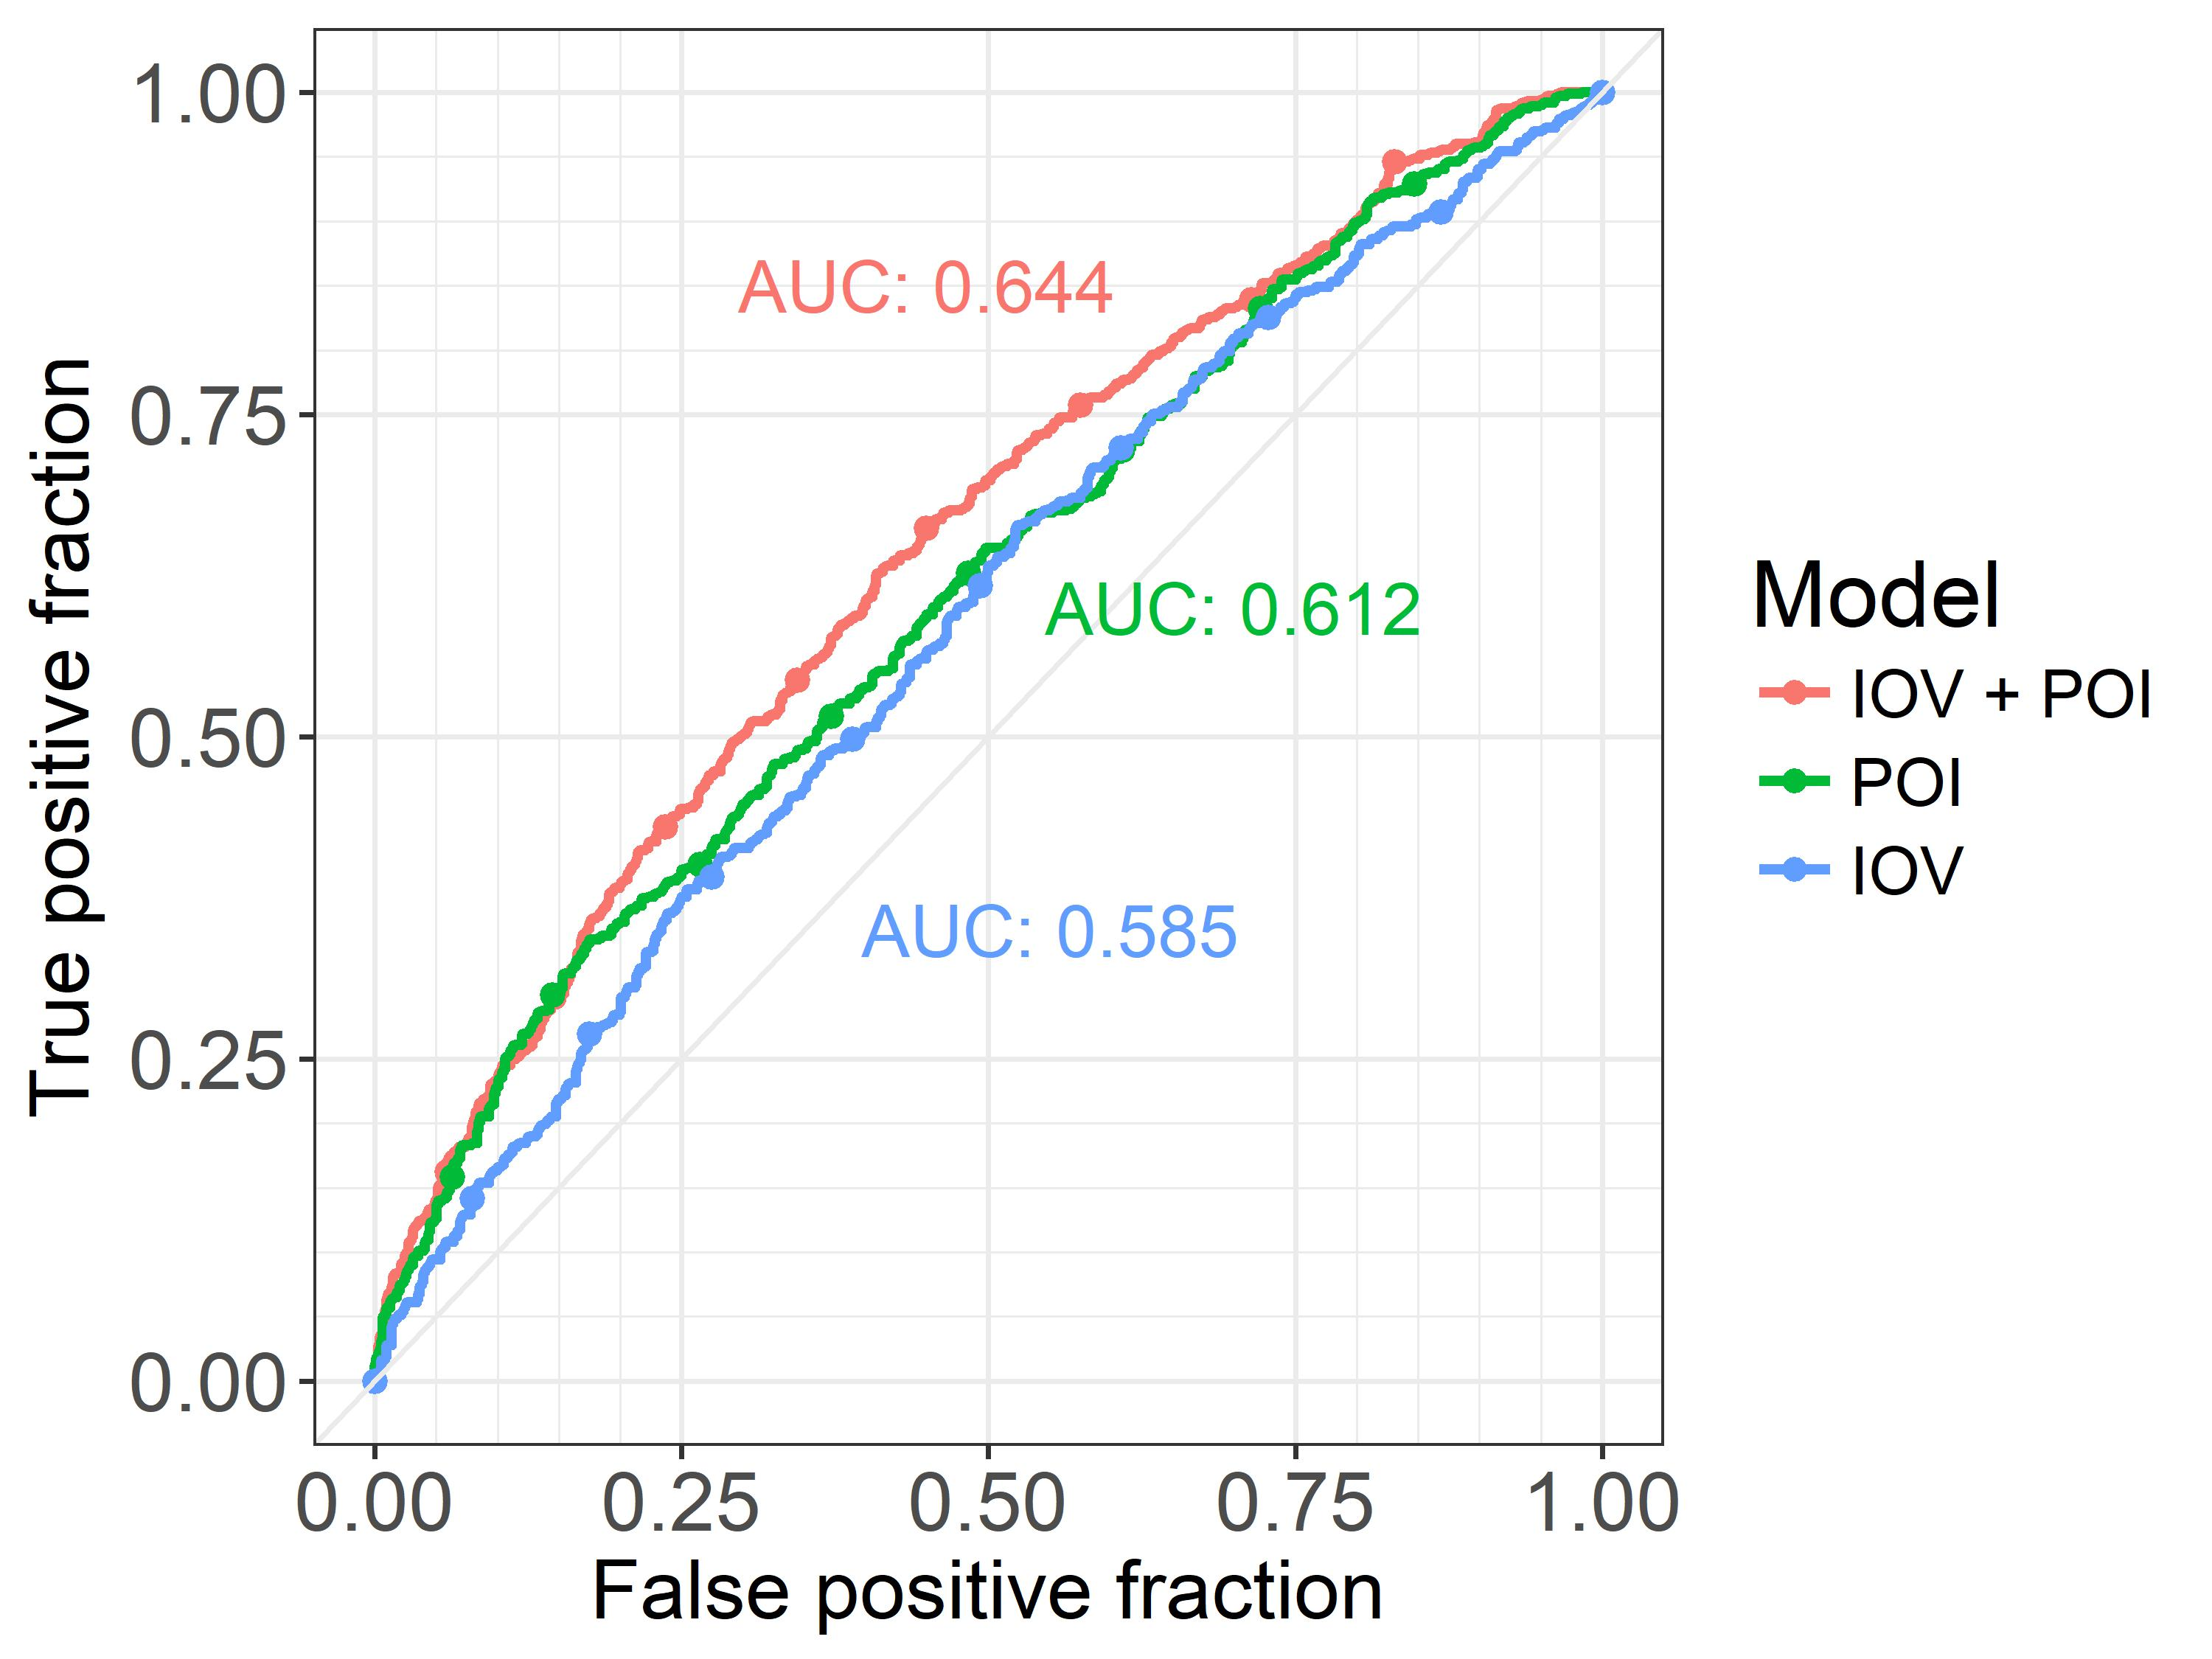
\includegraphics[width=0.937\linewidth]{ROC}
	\small\caption[]{Receiver operating characteristic curve of UBI model. The AUC of the UBI model is 0.644, while that of the model without POI or IOV data drops to 0.585 or 0.612.}
	\label{fig:ROC}
\end{figure}

\subsubsection{The POI predictors}
In order to derive 117 POI predictors, position of destination $\mathbf{d}_i^k \in \mathbb{R}^2$ for each vehicle $i$ in trip $k$ is first acquired, where $1 \leq k \leq t_i$, and elements in $\mathbf{d}_i^k$ represent latitude and longitude of destination. Let $B(\mathbf{d}_i^k , r)$ be the closed ball centered at $\mathbf{d}_i^k$ with radius $r > 0$. We then calculate
$$c_{ij}^k = \# \ of \ jth\ category \ POIs \ within \ B(\mathbf{d}_i^k , r),$$
where $r$ is 500 meters in this work. Finally, POI predictors $x_{ij}$ could be derived. That is, for $11 \leq j \leq 127$,
$$x_{ij}=\frac{\sum_{k=1}^{t_i} c_{ij}^k}{t_i}.$$
$x_{ij}$ could be interpreted as appearance frequencies of $j$th category POI for each vehicle $i$. It is shown in the data that mean frequency of all POI categories in all vehicles is 0.320, which indicates that each POI category appears 0.320 time on average in each trip. The most welcomed POI category is Residential area \& Restaurant with mean frequency of 3.422. On the contrary, the least welcomed one is Pet supply store \& Building gate with mean frequency of 0.001.


 
\begin{table*}[h]
 \centering
 \caption{Coefficient estimation of driving behavior predictors, the standard error and p-value are also reported}\label{tab:Result of Model Based on Driving Behavior Data} 
 \vspace{0.5ex}
 \begin{tabular}{llll}
  \toprule[1pt]
  \toprule[1pt]
  Predictor & Coefficient & Standard Error & p-value\\
  \midrule[1pt]
  Intercept & \ 0.062 &  0.093 & \  0.507\\
  $x_{i1}$ (Accumulative mileage) & \ 0.141& 0.060 & \ 0.018\\  
  $x_{i3}$ (Average fuel consumption) & -0.162 & 0.058 & \ 0.005\\
  $x_{i4}$ (Average engine rev) & -0.190 & 0.064 & \ 0.003\\
  $x_{i7}$ (Frequency of harsh braking) & \ 0.230 & 0.057 & \textless0.001\\
  \bottomrule[1pt]  
 \end{tabular}
\end{table*}


\subsection{Estimation Results}\label{UBI result}

IOV data and POI data are adopted to build the logistic regression model to score drivers. Bidirectional stepwise method with AIC was incorporated to conduct the model selection. In each step, the effect of eliminating or adding each predictor is evaluated by AIC. The selection will stop if adding or eliminating a predictor will cause larger AIC. After the model selection, $\hat{\beta}$ is derived from the model by maximum likelihood estimation method. Each driver was scored based on predicted probability of accident involvement. Then, the prediction result is assessed by Area Under Curve (AUC) which is widely adopted as an important indicator of prediction accuracy. Four of ten predictors besides POI predictors are included in the model, including accumulative mileage, average fuel consumption, average engine rev and frequency of harsh braking. They are represented in Table \ref{tab:Result of Model Based on Driving Behavior Data}. The coefficients of accumulative mileage and frequency of harsh braking are positive. While the coefficients of average fuel consumption and average engine rev represent that higher fuel consumption and engine rev are related to less possibility of accident. The sign of estimated coefficient of accumulative mileage is in accord with most previous literature. Other predictors are also easy to explain. Much harsh braking is related to less stability, and lower engine rev is a sign of low velocity and congestion, which might bring about more car accidents.


As for POI predictors, 22 POI predictors are incorporated in the UBI model. It is shown in the coefficients (Figure \ref{fig:coefficient}) that some POIs including Youth hotel and Museum \& Training organization contribute to the occurrence of accident. One likelihood is that roads around these places are commonly crowded especially on weekends so that complex traffic condition would bring about more accidents. Other POIs like III A hospital, Special hospital, and Mosque \& Tourism consultation are related to lower likelihood of being in accidents. It is conceivable that POIs like mosque are usually less crowded, and others like hospital are directed by more traffic wardens, which indicates fewer accidents.
%It is conceivable that these POIs usually are less crowded like mosque or directed by more traffic wardens like hospital, which indicates fewer accidents.


The AUC of the model is 0.644, while AUC of the model without POI data is 0.585 (Figure \ref{fig:ROC}). Obviously, POI data could be served as additional and informative predictors to improve the prediction result. In addition, the model could achieve high prediction accuracy even only with POI predictors, which is shown in Figure \ref{fig:ROC}. As it is stated above, POI data reflect driving habits of drivers and take the environment factor into consideration. Different POIs imply various preference that might be related to driving habits. Also, different POIs represent different traffic conditions and the risk of being involved in accidents. Thus, POI predictors present a new perspective on predicting accidents.

\subsection{Out-of-sample Result and Methods Comparison}
\begin{table*}[h]
	\centering
	\caption{Prediction accuracy of different methods on out-of-sample prediction. The average AUC or accuracy together with their standard deviation in 1000 times test is reported}\label{tab:methods comparison} 
	\vspace{0.5ex}
	\begin{tabular}{lllll|ll}
		\toprule[1pt]
		\toprule[1pt]
%		Variables used & Logistic Regression & Linear Discriminant Analysis & Quadratic Discriminant Analysis  & Deep Learning & Random Forest \\
		Predictors & Logistic Regression & LDA &	QDA  & Deep Learning & SVM & Random Forest \\
		\midrule[1pt]
		IOV & 0.576(0.022) & 0.577(0.022) & 0.559(0.024) & 0.573(0.024) & 0.547(0.020) & 0.537(0.021) \\
		IOV and POI & 0.608(0.022) & 0.611(0.021) & 0.567(0.023) & 0.600(0.024) & 0.570(0.020) & 0.547(0.022)\\  
		\cline{1-7}
		Improvement & 0.032 & 0.034 & 0.008 & 0.027 & 0.023 & 0.010\\
		\bottomrule[1pt]  
	\end{tabular}
\end{table*}

Logistic regression is one of the simplest but most powerful binary classifiers, which shows satisfactory prediction accuracy in Figure \ref{fig:ROC}.
There are two main reasons why logistic regression is adopted to build UBI model.
First, it is explicit in logistic regression model that how much certain driving behavior or POI contributes to the occurrence of accident. In application, this will help insurance companies understand the relationship between predictors and accidents.
%First of all, the form of logistic regression is straightforward and simple. Therefore, the model would be easily understood and mastered by actuaries. 
%Second, the output of logistic regression for new observation is predicted probability of accident rather than just predicted status. Predicted probability could offer more information for experienced actuaries than 0-1 result. Actuaries could adopt different methods based on the performance of predicted probability.

%Nevertheless, when classification accuracy is the only or main concern, logistic regression still achieve impressive accuracy compared with other probability-based or machine learning methods. 
Second, logistic regression achieves impressive accuracy compared with other classification methods.
In order to compare prediction accuracy of different methods, five another methods are adopted to build the UBI model, including LDA, QDA, multiple layer perception (deep learning), SVM and random forest. Specifically, the dataset are randomly divided into training set and test set in the ratio of 7 to 3. The model is first built on the training set and then classification accuracy is derived on the test set.  In order to rule out the effect of different predictors, predictors derived by stepwise logistic regression in subsection \ref{UBI result} are used in all methods. Each method is repeated 1000 times on both IOV data and full data set. Classification accuracy of methods that output 0-1 results (SVM and Random Forest) is evaluated by accuracy
$$A=\frac{\sum True\ Positive + \sum True\ Negative}{\sum Total\ Observation},$$ 
while the other's is evaluated by AUC.
It is shown in Table \ref{tab:methods comparison} that logistic regression, LDA and multiple layer perception methods perform satisfactorily in the measure of AUC, while other methods do not show obvious advantage over logistic regression. To sum up, in consideration of interpretability in real application and prediction accuracy, logistic regression is still recommended.





\section{Business Application}

\subsection{Driver Segmentation}
With more convenient and advancing facilitates to acquire IOV data, more and more insurance companies now offer UBI. However, POI data that are informative and easy to acquire have not been fully used of. The key of UBI is discerning drivers with different risk, and the accuracy of it could be improved by POI data. According to the model above with IOV and POI data, each driver could be scored based on $X_{i}^\top\hat{\beta}$ which is the predicted probability of getting involved in car accident. Furthermore, driver segmentation could be achieved according to the scores, and insurance companies could offer different premiums for drivers in different classes. To illustrate, we divide drivers in the dataset into four different risk classes as demonstrated in Figure \ref{fig:pred_group} and Figure \ref{fig:pred_group_q}. The accident risk of the first and the fourth classes are obviously different from those in other classes, so special premium strategy could be adapted to them in order to profit more in UBI market. For example, insurance companies could charge drivers in high-risk class higher premiums, while they can charge low-risk drivers less premiums to attract more customers. That strategy on average would reduce the premiums and profit more. Since the market of vehicle insurance is a fully developed market, this pricing advantage, despite tiny, would make great contribution. 

\begin{figure}[h!]
	\centering

	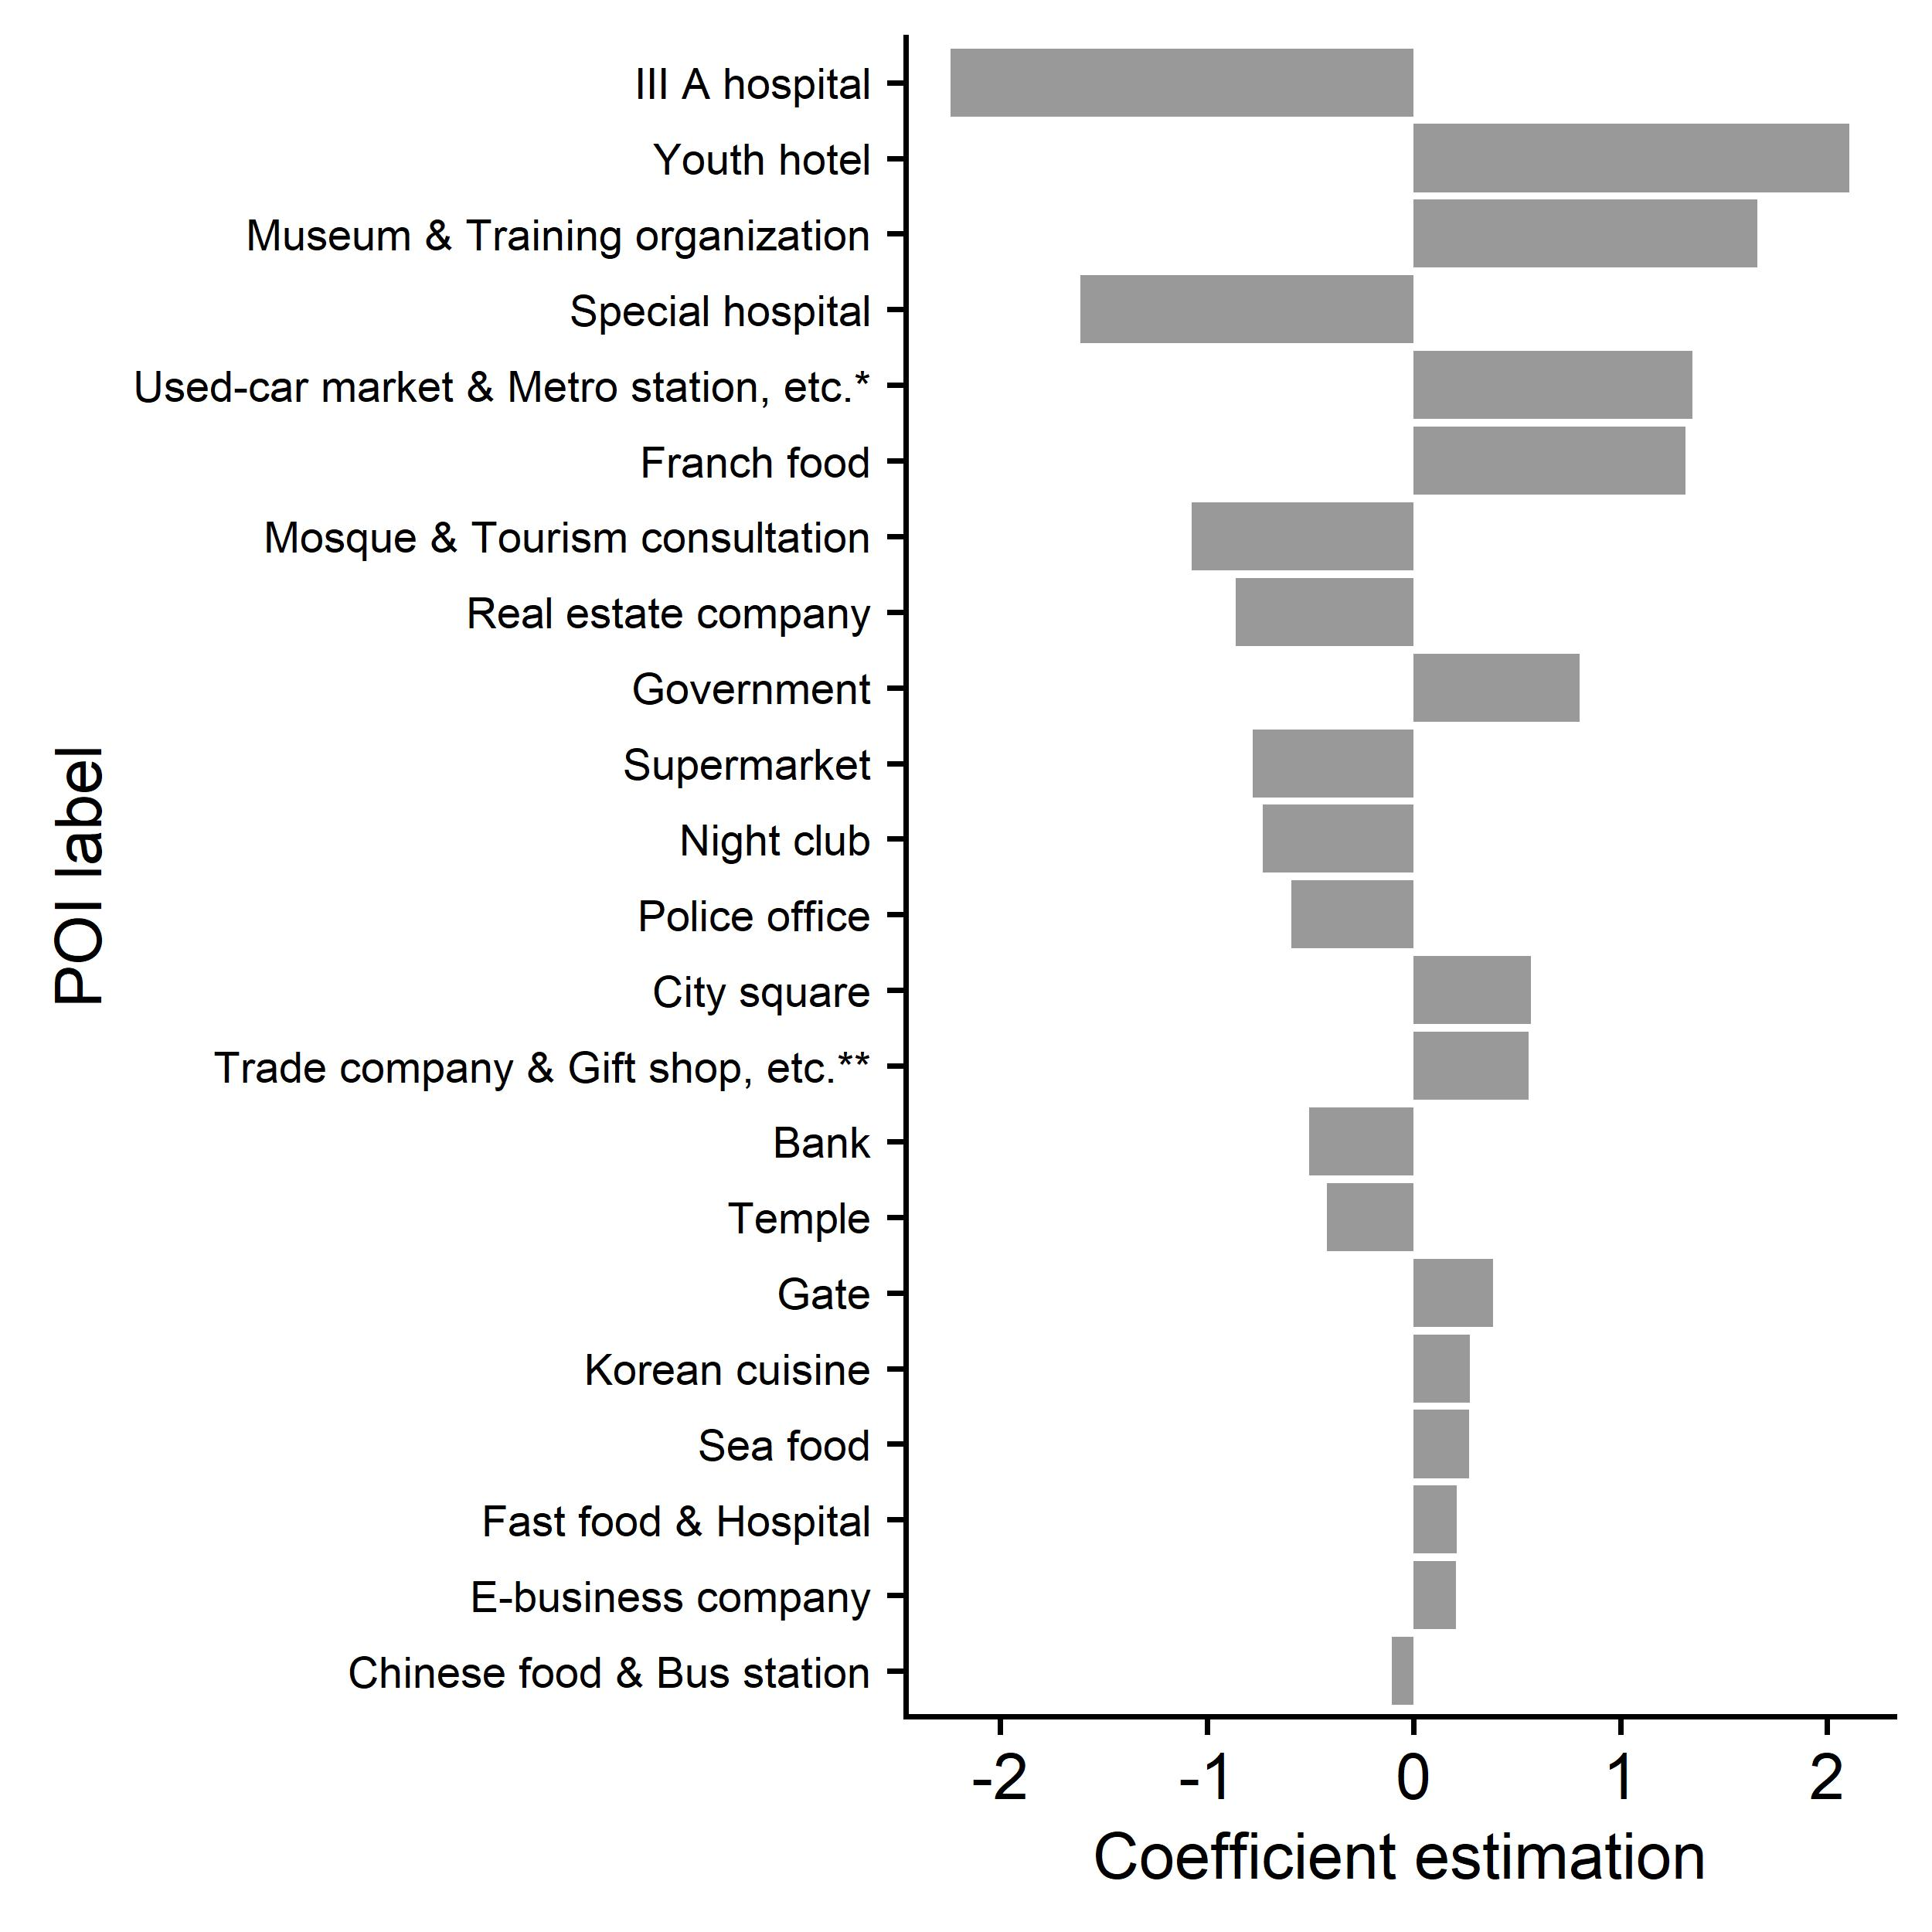
\includegraphics[width=1\linewidth]{coef}
	%\begin{minipage}{1cm}
    %\footnotesize
    %\emph{YOURNOTES}
    %\end{minipage}
	\caption*{\scriptsize*Full label is Used-car market \& Metro station \& Steak house \& Antique shop \& Hainan Cuisine \& Firehouse\\
	**Full label is Trade company \& Gift shop \& Press \& Casino }

	\small\caption[]{Coefficient estimation of POI predictors in UBI model. III A hospital is the POI predictor with the largest absolute value of coefficient.}
	\label{fig:coefficient}

\end{figure}

\begin{figure}[h]
	\centering
	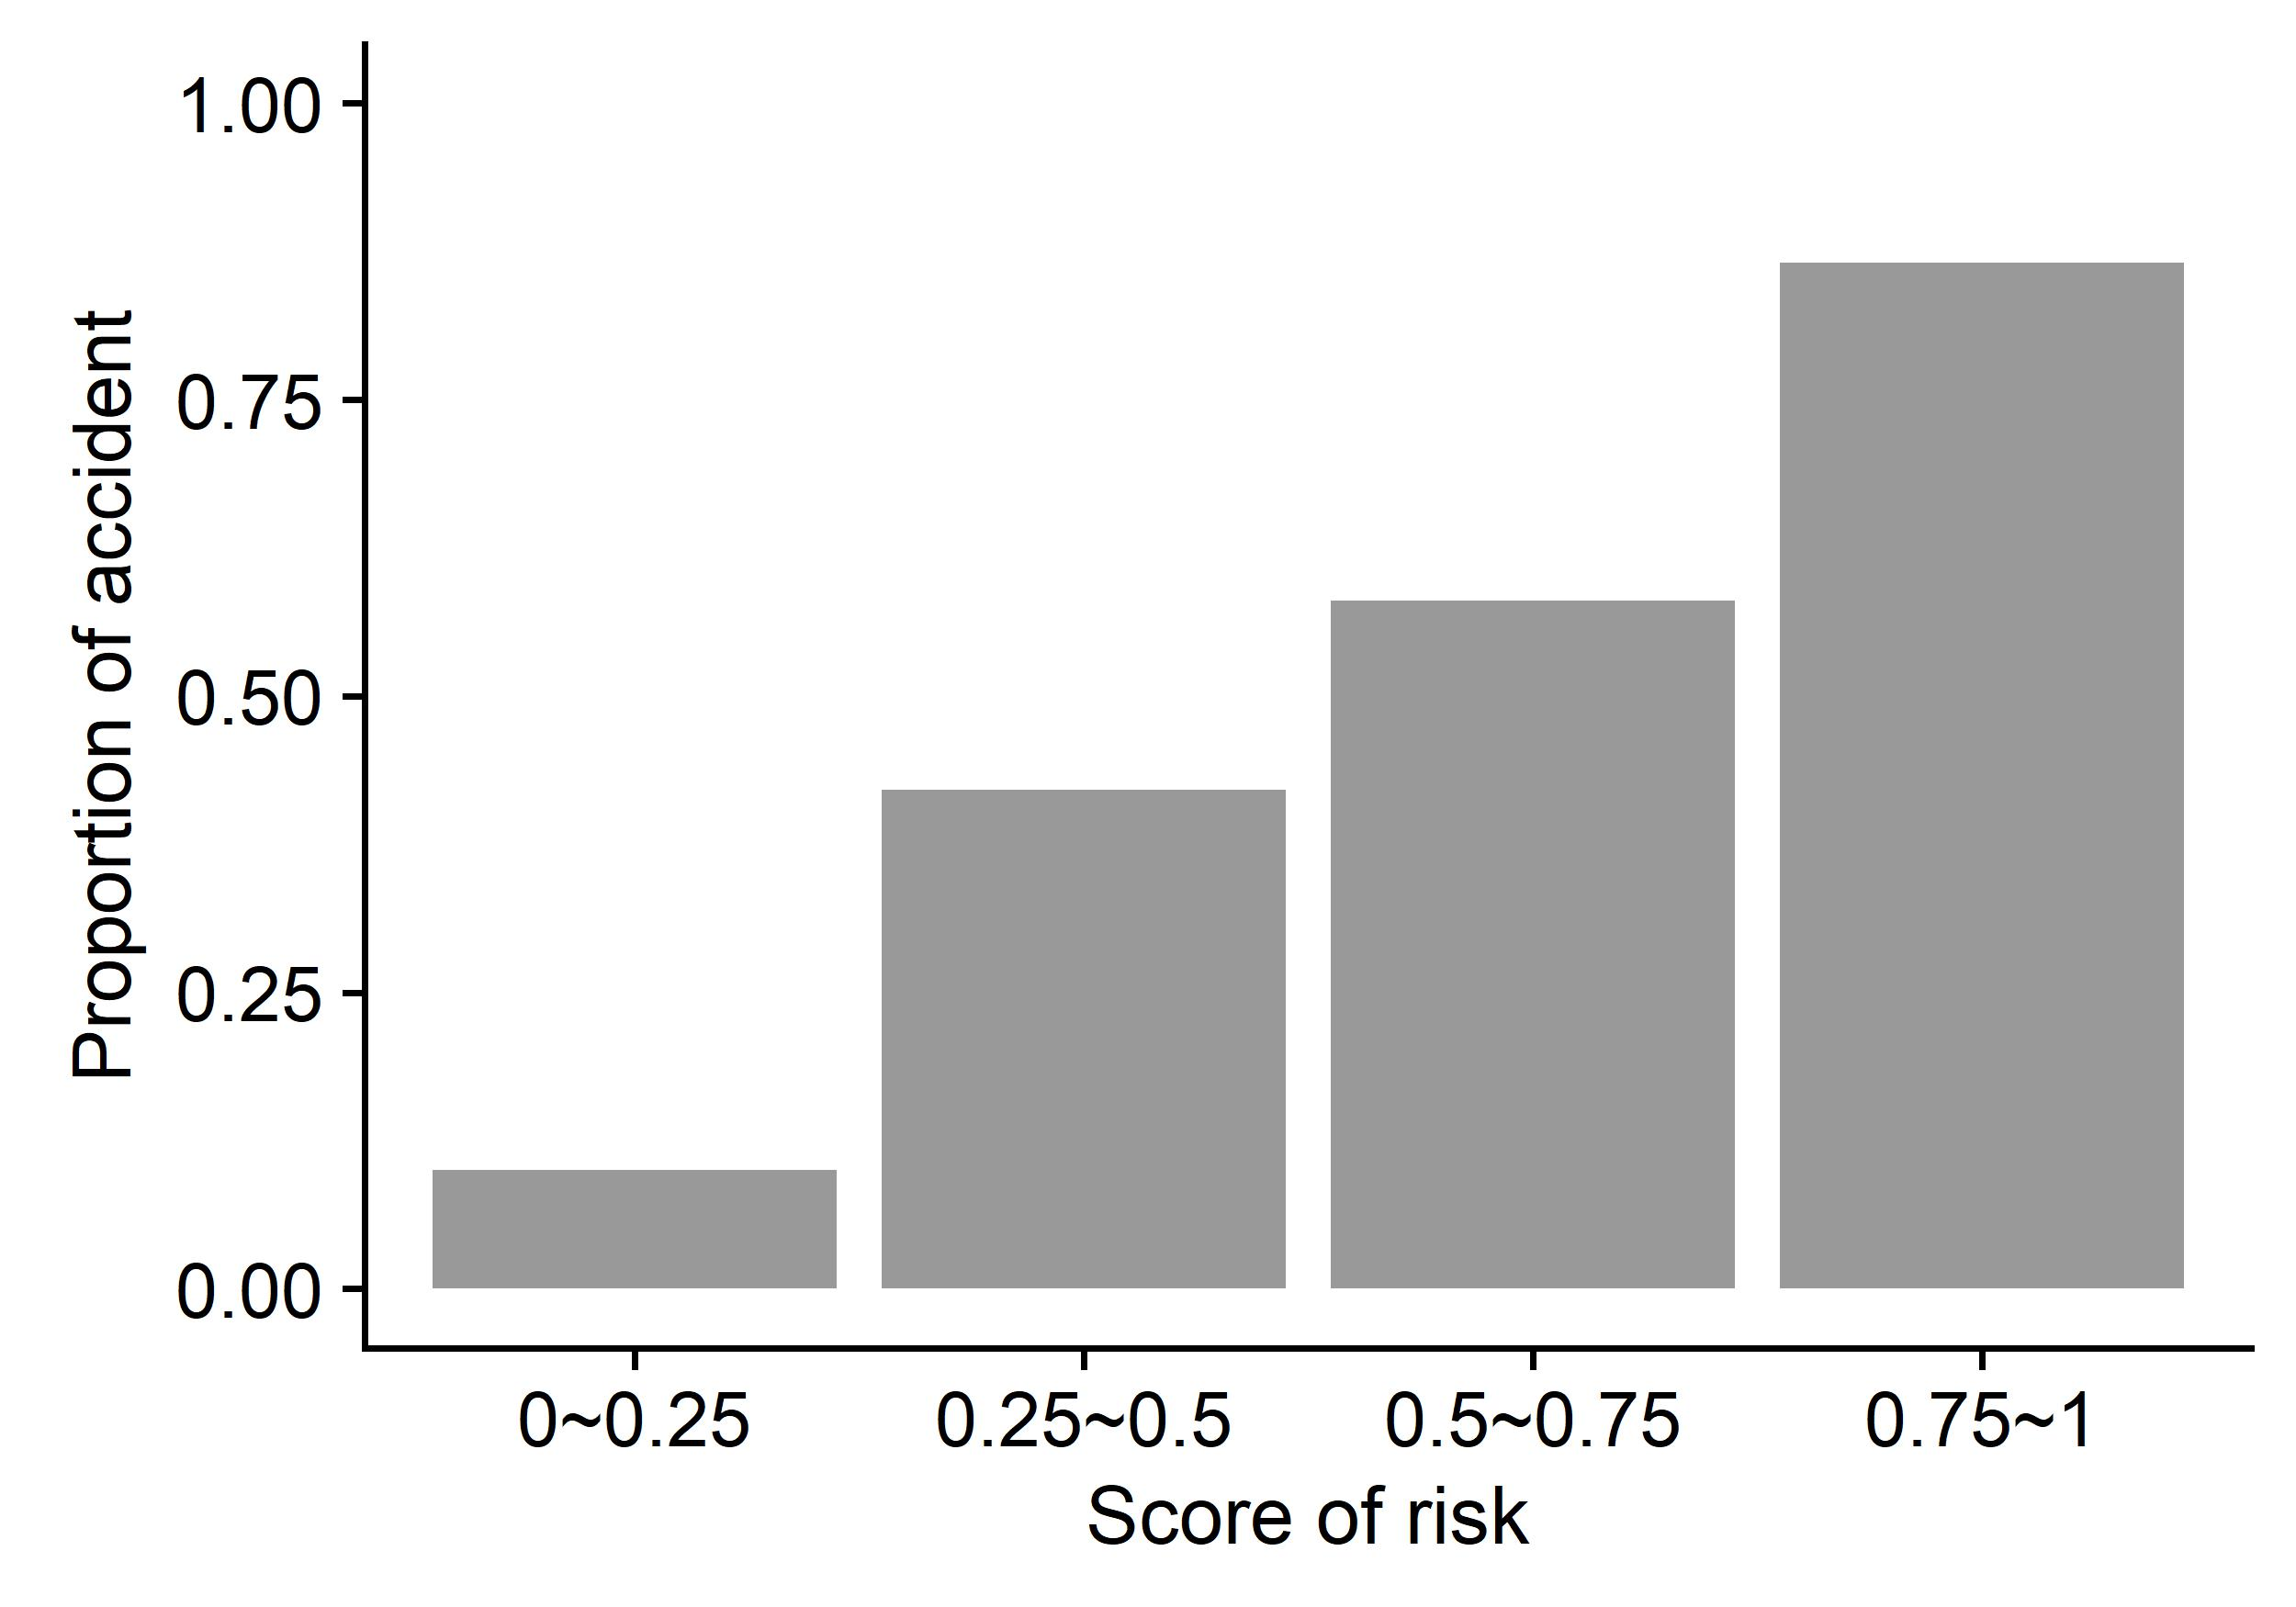
\includegraphics[width=0.99\linewidth]{pred_group}
	\small\caption[]{Proportion of accident in different groups according to scores of drivers. The predicted risk ranges are approximately in accord with actual proportion of accident.}
	\label{fig:pred_group}
\end{figure}

\begin{figure}[h!]
	\centering
	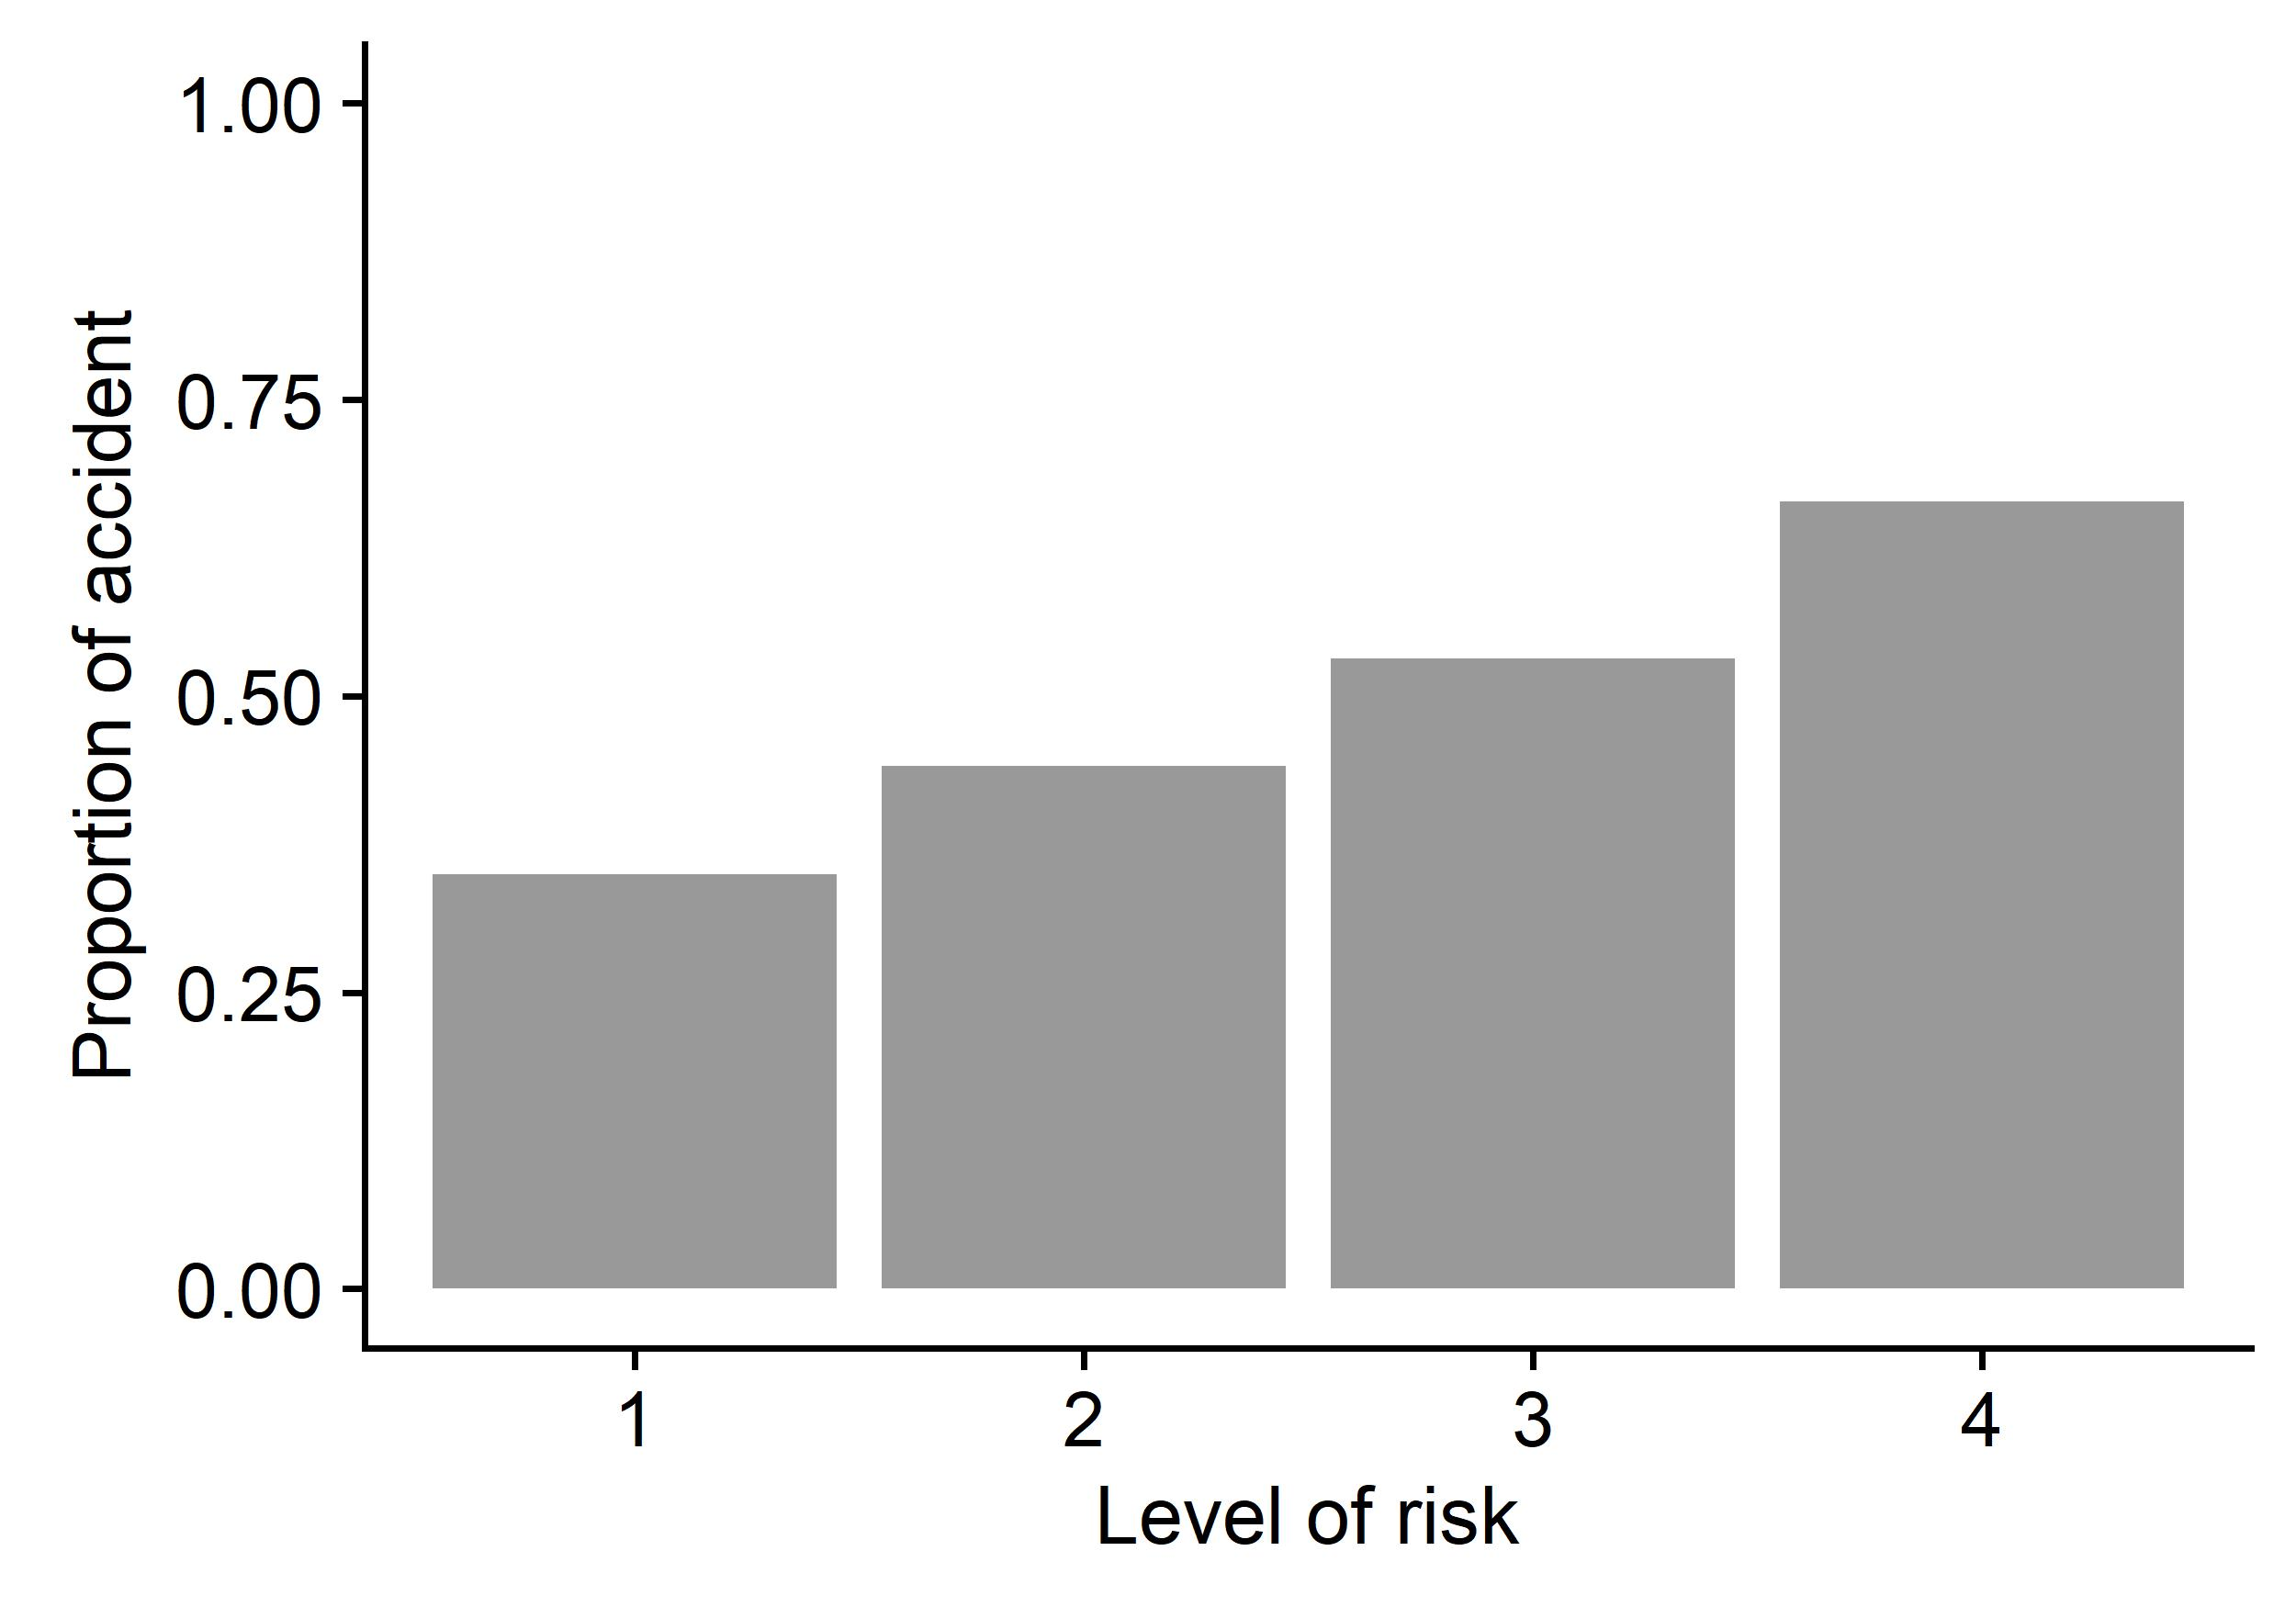
\includegraphics[width=1\linewidth]{pred_group_q}
	\small\caption[]{Different segmentation compared to the previous one. As the previous segmentation uses linear scores (actually, 0, 0.25, 0.75, and 1), this figure demonstrates the groups divided by quantiles to make size of each group similar.}
	\label{fig:pred_group_q}
\end{figure}

\subsection{Pricing Strategy}
There are mainly three UBI pricing options now, including mileage rate factor (MRF), per-mile premiums and GPS-based pricing. As for MRF, annual mileage served as a key rating factor in pricing. Drivers with low annual mileage will be provided with discount, and vice versa. GPS-based pricing uses IVDR to identify position of cars, and the premiums are based on when and where drivers drive. MRF only takes mileage into consideration and many MRF systems rely on self-reported estimates of future mileage, which might lead to less accuracy in pricing \cite{litman2008pay}.

Driving behavior rate factor (DBRF) which includes time, speed and other driving behavior serves as an expanded version of MRF, but the accuracy of DBRF can also be further improved \cite{liu2017risky}. By incorporating POI predictor into DBRF, more information about environment and driving habits are considered as it is shown in sections above. Based on driver segmentation result, linkage model could decide the rate adjustment coefficients based on scores of drivers \cite{liu2017risky}. Furthermore, the scores of drivers could be used for UBI pricing directly, since it not only reflects relative likelihood of accidents but also gives the probability of getting involved in an accident for each driver. 

\section{Concluding Remarks}
In this paper, we build a UBI model with IOV data and POI data. The data are collected by a major Chinese automobile manufacturer. Logistic regression model together with AIC is used to conduct the model selection. It is found that accumulative mileage, average fuel consumption, average engine rev, frequency of harsh braking and other 22 POI predictors are incorporated in the final model, which lead to an AUC of 0.644. In addition, the business application of the model in driver segmentation and UBI pricing is also discussed. To conclude this work, we have the following discussions about future research topics. First, the POI data are provided by Sina Weibo's open API, which are generated by its users. To further improve prediction accuracy, it is feasible to adopt a larger and more accurate POI dataset. Second, the UBI model takes insurance claim as response variable which is binary. Nonetheless, in practice, different accidents correspond to different amounts of compensation. So the amount of compensation and the type of accidents can be taken into consideration. Third, a threshold of 500 meters for scanning nearby POIs is set in our model for simplicity. As an alternative, it is more flexible to set the distance of scanning as a tuning parameter.



\newpage
\bibliographystyle{unsrt}	
\bibliography{essaybib} 


\end{document}


